\documentclass[letterpaper,journal]{IEEEtran}
\usepackage{amsmath,amsfonts}
\usepackage{algorithmic}
\usepackage{algorithm}
\usepackage{array}
\usepackage[caption=false,font=normalsize,labelfont=sf,textfont=sf]{subfig}
\usepackage{textcomp}
\usepackage{stfloats}
\usepackage{url}
\usepackage{verbatim}
\usepackage{graphicx}
\usepackage{cite}
\usepackage{placeins}
\usepackage{booktabs}

% highlights
\usepackage[dvipsnames,svgnames,x11names]{xcolor}
\usepackage{soul}    % for text highlight
\soulregister\cite7  % so that \cite doesn't break highlighting
\soulregister\ref7   % so that \ref doesn't break highlighting


\hyphenation{op-tical net-works semi-conduc-tor IEEE-Xplore}
% updated with editorial comments 8/9/2021

\begin{document}

\title{Performance Evaluation of Post-Quantum Cryptographic Algorithms on C-V2X Sidelink Communications}

\author{%
Akid Abrar,~\IEEEmembership{Student Member,~IEEE},
Sagar Dasgupta,
Abdullah Al Mamun,
Mizanur Rahman,~\IEEEmembership{Senior Member,~IEEE},
Ahmad Alsharif,
and Mashrur Chowdhury

\thanks{Akid Abrar, Sagar Dasgupta,Ahmad Alsharif and Mizanur Rahman are with the Department of Civil, Construction \& Environmental Engineering, The University of Alabama, Smart Communities and Innovation Building (SCIB), 28 Kirkbride Lane, Tuscaloosa, AL 35487-0288 USA (emails: aabrar@crimson.ua.edu; sdasgupta@ua.edu; mizan.rahman@ua.edu; aalsharif1@ua.edu.).}%
\thanks{Abdullah Al Mamun and Mashrur Chowdhury are with the Glenn Department of Civil Engineering, Clemson University, Clemson, SC 29634 USA. (emails: abdullm@clemson.edu; mac@clemson.edu).}%
\thanks{Copyright (c) 20xx IEEE. Personal use of this material is permitted. However, permission to use this material for any other purposes must be obtained from the IEEE by sending a request to pubs-permissions@ieee.org.}
}

% The paper headers
% \markboth{Journal of \LaTeX\ Class Files,~Vol.~14, No.~8, August~2021}%
% {Shell \MakeLowercase{\textit{et al.}}: A Sample Article Using IEEEtran.cls for IEEE Journals}

\IEEEpubid{0000--0000/00\$00.00~\copyright~2025 IEEE}
% Remember, if you use this you must call \IEEEpubidadjcol in the second
% column for its text to clear the IEEEpubid mark.


\maketitle

\begin{abstract}
Wireless connectivity, such as Cellular-Vehicle-to-Everything (C-V2X), between vehicles and transportation infrastructure promises significant roadway safety benefits by providing 360-degree views of their surroundings. However, wireless connectivity in intelligent transportation systems is vulnerable to deliberate cyber threats. Security of wireless connectivity relies on traditional cryptographic techniques as specified in the IEEE 1609.2 standard. The anticipated advent of quantum computing can compromise this cryptographic foundation. Post-quantum cryptographic (PQC) algorithms offer quantum-resistant alternatives. However, the significantly larger size of PQC signatures and public keys poses a challenge to meet communication latency for safety-critical transportation applications. This study conducts a comprehensive evaluation of standardized PQC algorithms on C-V2X sidelink performance to assess the feasibility of implementing PQC in safety-critical transportation applications. C-V2X sidelink key performance indicators (KPIs), including packet delivery ratio (PDR), end-to-end latency, channel busy ratio (CBR), and resource utilization, are compared across PQC algorithms at varying levels of service at an urban roadway intersection to confirm their applicability.

\end{abstract}

\begin{IEEEkeywords}
C-V2X, post-quantum cryptography, sidelink, Mode~4, Falcon-512, ECDSA, IEEE~1609.2, SAE~J3161, vehicle-to-everything
\end{IEEEkeywords}

\section{Introduction}
\IEEEPARstart{C}{ellular} Vehicle-to-Everything (C-V2X) communication enables vehicles to exchange safety-critical messages such as Basic Safety Messages (BSMs) over the PC5 sidelink interface at 10~Hz, providing each vehicle with a 360-degree awareness of its surrounding traffic environment~\cite{molina2017lte}. The C-V2X Mode~4 sidelink, standardized by 3GPP in Release~14 and profiled for deployment by SAE~J3161~\cite{sae_j3161}, operates without cellular infrastructure by allowing vehicles to autonomously select radio resources through a sensing-based Semi-Persistent Scheduling (SPS) mechanism. This infrastructure-independent operation makes Mode~4 particularly attractive for safety applications in areas lacking network coverage, such as rural highways and intersection approaches.

The integrity and authenticity of V2X messages are ensured through digital signatures as specified in the IEEE~1609.2 security standard~\cite{ieee_16092}. Currently, IEEE~1609.2 mandates the Elliptic Curve Digital Signature Algorithm (ECDSA) with the NIST P-256 curve, which produces compact 64-byte signatures and 65-byte public keys. These sizes impose minimal overhead on the sidelink transport block, and the V2X ecosystem, including the Security Credential Management System (SCMS)~\cite{brecht2018scms}, which has been designed around these compact parameters.

However, the anticipated emergence of cryptographically relevant quantum computers poses a fundamental threat to elliptic-curve-based cryptography. Shor's algorithm~\cite{shor1994algorithms} can solve the elliptic curve discrete logarithm problem in polynomial time, rendering ECDSA insecure. While the timeline for such quantum capabilities remains uncertain, the long deployment lifecycle of transportation infrastructure (15--20~years for vehicles and roadside equipment) demands proactive migration planning~\cite{campagna2020pqc_migration}. The National Institute of Standards and Technology (NIST) has responded by standardizing post-quantum cryptographic (PQC) algorithms resistant to quantum attacks, including lattice-based digital signature schemes such as ML-DSA (Dilithium, FIPS~204)~\cite{fips204} and FN-DSA (Falcon, FIPS~206)~\cite{fips206}.

The central challenge in adopting PQC for V2X lies in the significantly larger signature and public key sizes of post-quantum algorithms. Falcon-512, the most compact NIST PQC signature scheme, produces signatures of 649--666~bytes and public keys of 897~bytes, an order of magnitude larger than ECDSA. Dilithium-2 is even larger, with 2420-byte signatures and 1312-byte public keys. These inflated sizes directly increase the Secure Protocol Data Unit (SPDU) payload that must be accommodated within the C-V2X sidelink transport block, which is constrained by the Message Coding Scheme (MCS) index, subchannel allocation, and congestion control parameters mandated by SAE~J3161. Whether the sidelink can accommodate this overhead without degrading safety-critical KPIs such as packet delivery ratio and latency remains an open question that we aim to address in this study.
\IEEEpubidadjcol
Existing studies on PQC in vehicular contexts have focused primarily on computational benchmarking on embedded hardware~\cite{kumar2024pqc_automotive} or on abstract protocol-level analysis without considering the radio resource constraints of the C-V2X physical layer. To the best of the authors' knowledge, no prior work has evaluated the end-to-end impact of PQC digital signatures on C-V2X Mode~4 sidelink performance within a standards-compliant simulation environment that models the full protocol stack from application-layer signing through MAC-layer resource allocation to physical-layer transmission. The key contributions of this study are as follows:
\begin{itemize}
    \item This study presents the first implementation and evaluation of NIST-standardized PQC digital signature algorithms within a C-V2X PC5 Mode~4 sidelink simulation that maintains compliance with SAE~J3161 deployment parameters and IEEE~1609.2 security standards.
    \item A feasibility assessment is conducted to determine whether PQC algorithms can be adopted without modifications to the application layer (e.g., packet segmentation or hybrid cryptographic schemes) or to the lower-layer radio resource configuration (e.g., MCS adaptation beyond the J3161-specified range).
    \item A cross-layer performance evaluation quantifies the impact of PQC signature and public key overhead on sidelink KPIs, including PDR, signature generation and verification time, end-to-end latency, CBR, and subchannel resource utilization.
    \item Multiple urban intersection scenarios with varying vehicle densities (levels of service) are evaluated to identify the density thresholds at which PQC-induced overhead begins to degrade sidelink performance relative to the incumbent ECDSA baseline.
\end{itemize}

The remainder of this paper is organized as follows. Section~\ref{sec:background} provides background on C-V2X Mode~4 sidelink and security standards along with PQC algorithms. Section~\ref{sec:related} reviews related work. Section~\ref{sec:method} describes the simulation methodology and setup. Section~\ref{sec:results} presents the evaluation outcomes. Section~\ref{sec:discussion} discusses the findings and their implications, and Section~\ref{sec:conclusion} concludes the paper.

%%%%%%%%%%%%%%%%%%%%%%%%%%%% SECTION %%%%%%%%%%%%%%%%%%%%%%%%%%%%%%%%%%%%%%%
\section{Background}
\label{sec:background}

%%%%%%%%%%%%%%%%%%%%%% SUBSECTION %%%%%%%%%%%%%%%%%%%%%%
\subsection{C-V2X Mode~4 and SAE J3161}
\label{sec:cv2x}

C-V2X is a 3GPP-standardized radio access technology that enables direct vehicle-to-vehicle (V2V) communication over the PC5 sidelink interface without requiring cellular network infrastructure~\cite{3gpp_36213}. The PC5 interface operates in the 5.9~GHz Intelligent Transportation Systems (ITS) band and supports two transmission modes: Mode~3, where a base station schedules sidelink resources, and Mode~4, where vehicles autonomously select resources using a sensing-based Semi-Persistent Scheduling (SPS) mechanism~\cite{molina2017lte}.

In Mode~4, each vehicle monitors the sidelink spectrum over a sensing window of 1000~ms and identifies candidate single-subframe resources within a selection window. Resources whose received power exceeds a threshold (Reference Signal Received Power, RSRP) are excluded from the candidate set. The vehicle then randomly selects a resource from the remaining candidates and reserves it for a configurable Resource Reservation Interval (RRI). A reselection counter determines how many consecutive transmissions use the reserved resource before triggering a new selection~\cite{3gpp_36321}. At each reselection event, the vehicle retains the current resource with a probability $p_\text{keep}$ (typically 0.0, 0.2, 0.4, 0.6, or 0.8) or selects a new resource from the updated candidate set.

The transmission payload is carried on the Physical Sidelink Shared Channel (PSSCH), while the associated Sidelink Control Information (SCI) is transmitted on the Physical Sidelink Control Channel (PSCCH). Adjacent PSCCH--PSSCH mapping is typically employed, where control and data subchannels occupy contiguous resource blocks within the same subframe. The Modulation and Coding Scheme (MCS) applied to the PSSCH determines the transport block size and, consequently, the maximum payload that can be accommodated within a given number of subchannels.

SAE~J3161~\cite{sae_j3161} specifies the deployment profile for C-V2X V2V communication in the 5.9~GHz band. It mandates a 10~MHz channel bandwidth corresponding to 50 resource blocks per subframe, a subchannel size of 10 or 20 resource blocks, and an RRI of 100~ms aligned with the Basic Safety Message (BSM) generation rate specified in SAE~J2945/1. The standard further defines congestion control through Channel Busy Ratio (CBR) monitoring and specifies MCS ranges and maximum subchannel allocations as a function of measured CBR. These constraints collectively determine the maximum packet size that the sidelink can carry, which directly impacts the feasibility of deploying cryptographic algorithms with large signature and key sizes.

%%%%%%%%%%%%%%%%%%%%%% SUBSECTION %%%%%%%%%%%%%%%%%%%%%%
\subsection{Post-Quantum Cryptography}
\label{sec:pqc}

Current V2X security, as specified in IEEE~1609.2~\cite{ieee_16092}, relies on the Elliptic Curve Digital Signature Algorithm (ECDSA) with the NIST P-256 curve for message authentication. An ECDSA P-256 signature is 64~bytes (raw $r \| s$ format), and the corresponding public key is 65~bytes (uncompressed point), resulting in modest overhead that is readily accommodated within the sidelink transport block~\cite{ieee_16092}.

The anticipated advent of large-scale quantum computers threatens to break ECDSA and other elliptic-curve-based schemes through Shor's algorithm~\cite{shor1994algorithms}. In response, the National Institute of Standards and Technology (NIST) conducted a multi-year standardization process and selected several post-quantum cryptographic algorithms for standardization~\cite{nist_pqc_report}. Among the digital signature schemes, two are particularly relevant to V2X applications:

\textbf{ML-DSA (Dilithium).} ML-DSA, formerly known as CRYSTALS-Dilithium, is a lattice-based digital signature scheme standardized as FIPS~204~\cite{fips204}. At security level~2, Dilithium-2 produces signatures of 2420~bytes with a public key of 1312~bytes. While Dilithium offers strong security guarantees and deterministic signing, its signature and key sizes are substantially larger than ECDSA.

\textbf{FN-DSA (Falcon).} FN-DSA, formerly known as Falcon, is a lattice-based signature scheme based on NTRU lattices and fast Fourier sampling, standardized as FIPS~206~\cite{fips206}. Falcon-512 produces compact signatures of approximately 649--666~bytes (variable length) with a public key of 897~bytes. Falcon offers the smallest combined signature and key size among the NIST-selected PQC signature schemes, making it the most promising candidate for bandwidth-constrained applications such as V2X sidelink.

Table~\ref{tab:crypto_sizes} summarizes the signature and public key sizes for the three algorithms evaluated in this study.

\begin{table}[!htbp]
    \caption{Cryptographic Algorithm Parameter Sizes}
    \label{tab:crypto_sizes}
    \centering
    \begin{tabular}{lccc}
    \toprule
    \textbf{Algorithm} & \textbf{Signature (B)} & \textbf{Public Key (B)} & \textbf{Security Level} \\
    \midrule
    ECDSA P-256    & 64        & 65      & Classical 128-bit \\
    Falcon-512     & 649--666  & 897     & NIST Level~1 \\
    Dilithium-2    & 2420      & 1312    & NIST Level~2 \\
    \bottomrule
    \end{tabular}
\end{table}

%%%%%%%%%%%%%%%%%%%%%%%%%%%% SECTION %%%%%%%%%%%%%%%%%%%%%%%%%%%%%%%%%%%%%%%
\section{Related Work}
\label{sec:related}

Prior research related to this study can be categorized into three areas: (1)~C-V2X Mode~4 sidelink performance evaluation, (2)~V2X security and IEEE~1609.2 authentication overhead, and (3)~post-quantum cryptography for vehicular and IoT systems.

\subsection{C-V2X Mode~4 Performance Evaluation}

Several studies have evaluated the performance of LTE-V2X Mode~4 sidelink communication through analytical modeling and simulation. Gonzalez-Martin et al.~\cite{gonzalez2019analytical} developed analytical models to characterize Mode~4 PDR as a function of vehicle density, demonstrating that the SPS mechanism can sustain high reliability at low-to-moderate densities but degrades under congestion due to persistent packet collisions. Bazzi et al.~\cite{bazzi2017performance} compared IEEE~802.11p and LTE-V2V performance, showing that C-V2X achieves superior range and reliability under highway scenarios. McCarthy et al.~\cite{mccarthy2020opencvx} introduced openCV2X, the first open-source Mode~4 simulation model built on SimuLTE and OMNeT++, and demonstrated its cross-layer fidelity for evaluating aperiodic traffic patterns. Toghi et al.~\cite{toghi2019congestion} analyzed Mode~4 performance under highly congested conditions, highlighting the role of CBR-based congestion control in maintaining channel stability. These studies collectively establish the baseline performance characteristics of Mode~4 sidelink; however, none of them incorporate the impact of cryptographic overhead on sidelink KPIs.

\subsection{V2X Security and Authentication Overhead}

The IEEE~1609.2 standard~\cite{ieee_16092} defines the security services for V2X, including ECDSA-based digital signatures and a certificate management framework. Qu et al.~\cite{qu2015security} provided a comprehensive review of VANET security challenges, identifying message authentication as a key bottleneck for high-frequency BSM transmission. Brecht et al.~\cite{brecht2018scms} described the SCMS architecture for V2X certificate management in the United States, noting that the system was designed around the compact size of ECDSA P-256 credentials. Lu et al.~\cite{lu2018survey_v2x_security} surveyed security and privacy for 5G V2X, emphasizing that any migration to new cryptographic primitives must satisfy the strict latency requirements of safety-critical applications. While these works thoroughly address the security architecture, they do not evaluate the radio resource impact of alternative cryptographic algorithms on the sidelink physical layer.

\subsection{Post-Quantum Cryptography for Vehicular Systems}

The application of PQC to vehicular systems has received growing attention following the NIST standardization process. Fernandez et al.~\cite{fernandez2023pqc_v2x} reviewed post-quantum approaches for securing vehicular blockchain systems, identifying Falcon as a promising candidate due to its compact signature size. Kumar et al.~\cite{kumar2024pqc_automotive} benchmarked PQC algorithms on automotive-grade embedded platforms, demonstrating that Falcon-512 signing completes in approximately 0.21~ms and verification in 0.05~ms on ARM processors, while Dilithium-2 exhibits comparable verification times but larger signatures. Hasan et al.~\cite{hasan2022pqc_v2v} proposed a practical post-quantum authentication framework for V2V, evaluating Falcon and Dilithium in terms of computational cost but without modeling their impact on the radio access layer. Shen et al.~\cite{shen2025pqc_analysis} analyzed PQC signature performance for intelligent transportation systems, providing an implementation-focused review that highlighted the tension between PQC key sizes and the bandwidth limitations of vehicular communication channels. A recent SAE technical paper~\cite{sae2026pqc_twowheeler} evaluated PQC feasibility on embedded systems for two-wheeler security, confirming that computational overhead is manageable on modern hardware but leaving radio resource impact unexamined.

\subsection{Research Gap}

While existing literature has separately addressed C-V2X Mode~4 sidelink performance, V2X security frameworks, and PQC algorithm benchmarking, no prior study has jointly evaluated these aspects within a single, standards-compliant simulation. Specifically, the impact of PQC signature and key sizes on sidelink radio resource allocation, packet delivery, and latency under realistic SAE~J3161 deployment parameters has not been quantified. This study addresses this gap by implementing PQC algorithms within a full-stack C-V2X Mode~4 simulator and evaluating their end-to-end impact on sidelink KPIs across varying traffic densities.

%%%%%%%%%%%%%%%%%%%%%%%%%%%% SECTION %%%%%%%%%%%%%%%%%%%%%%%%%
\section{Methodology}
\label{sec:method}

This section describes the simulation framework, the traffic scenarios, the IEEE~1609.2-compliant packet structure, and the KPIs used for evaluation.

%%%%%%%%%%%%%%%%%%%%%% SUBSECTION %%%%%%%%%%%%%%%%%%%%%%
\subsection{Simulation Framework}
\label{sec:sim_framework}

The simulation environment is built upon the openCV2X implementation of SimuLTE~\cite{virdis2014simulte}, an open-source C-V2X simulator developed for the OMNeT++ discrete-event simulation platform~\cite{varga2019omnetpp}. openCV2X models the full LTE protocol stack, including the physical layer, MAC layer with Mode~4 SPS resource allocation, RLC, and PDCP layers. The simulator is coupled with Veins~\cite{sommer2019veins} for vehicular networking abstractions and with SUMO (Simulation of Urban MObility)~\cite{lopez2018sumo} for realistic microscopic traffic simulation.

The sidelink physical layer is configured with a carrier frequency of 5915~MHz in the 5.9~GHz ITS band. The channel bandwidth is 20 MHz, providing 100 resource blocks per subframe in the uplink. A subchannel size of 10 resource blocks is used, yielding 10 subchannels per subframe. The MCS index ranges from 5 to 11, consistent with the SAE~J3161 deployment profile. Preconfigured transmission parameters are used, and CBR-based congestion control with channel occupancy ratio (CR) limiting is enabled. Each vehicle transmits at 23~dBm and reserves resources with an RRI of 100~ms. The resource keep probability is set to $p_\text{keep} = 0.8$, and the RSSI-based sensing threshold is 9~dB.

The PQC algorithms are implemented using the liboqs library~\cite{stebila2020liboqs}, which provides reference implementations of NIST-standardized post-quantum algorithms. ECDSA P-256 is implemented using OpenSSL. Each vehicle and RSU generates a fresh key pair at initialization and performs real-time signing and verification of every BSM, capturing actual computational overhead in the simulation timing.

Table~\ref{tab:sim_params} summarizes the key simulation parameters.

\begin{table}[!htbp]
    \caption{Simulation Parameters}
    \label{tab:sim_params}
    \centering
    \begin{tabular}{lc}
    \toprule
    \textbf{Parameter} & \textbf{Value} \\
    \midrule
    Carrier frequency          & 5915~MHz \\
    Channel bandwidth          & 20~MHz \\
    Number of resource blocks  & 100 per subframe \\
    Subchannel size            & 10~RBs \\
    Number of subchannels      & 10 \\
    MCS range                  & 5--11 \\
    Transmit power             & 23~dBm \\
    Resource reservation interval (RRI) & 100~ms \\
    Resource keep probability ($p_\text{keep}$) & 0.8 \\
    RSSI sensing threshold     & 9~dB \\
    BSM generation rate        & 10~Hz (100~ms) \\
    Simulation duration        & 60~s \\
    Congestion control         & CBR-based with CR limiting \\
    HARQ retransmissions       & 0 \\
    Cryptographic library (PQC)  & liboqs \\
    Cryptographic library (ECDSA) & OpenSSL \\
    Traffic simulator          & SUMO \\
    \bottomrule
    \end{tabular}
\end{table}

%%%%%%%%%%%%%%%%%%%%%% SUBSECTION %%%%%%%%%%%%%%%%%%%%%%
\subsection{IEEE 1609.2 Compliant Packet Structure}
\label{sec:packet_structure}

Each transmitted packet follows the IEEE~1609.2 SPDU structure~\cite{ieee_16092}. The SPDU encapsulates a J2735 BSM Part~I (BSMcoreData), which contains vehicle position, speed, heading, and other kinematic data totaling 39~bytes per the J2735 standard~\cite{sae_j2735}.

The IEEE~1609.2 \texttt{Ieee1609Dot2Data} wrapper adds a protocol version, content type, hash algorithm identifier, Provider Service Identifier (PSID), generation time, generation location, and encoding overhead, contributing approximately 28~bytes of fixed overhead. The \texttt{SignerIdentifier} field alternates between including the full explicit certificate and a compact \texttt{HashedId8} digest (8~bytes), following the certificate inclusion strategy specified in SAE~J2945/1~\cite{sae_j29451}. When the full certificate is included, it comprises a fixed overhead of approximately 105~bytes (version, type, issuer identifier, validity period, application permissions, and verification key indicator) plus the raw public key of the signing algorithm.

The total SPDU size for each algorithm, when transmitting with a full certificate, is:
\begin{equation}
    S_\text{SPDU} = S_\text{hdr} + S_\text{BSM} + S_\text{sig} + S_\text{cert}
    \label{eq:spdu_size}
\end{equation}
where $S_\text{hdr} = 28$~bytes is the IEEE~1609.2 header overhead, $S_\text{BSM} = 39$~bytes is the BSM payload, $S_\text{sig}$ is the digital signature size, and $S_\text{cert} = 105 + S_\text{pk}$ is the certificate size including the raw public key. Table~\ref{tab:spdu_sizes} presents the resulting SPDU sizes.

\begin{table}[!htbp]
    \caption{SPDU Sizes with Full Certificate}
    \label{tab:spdu_sizes}
    \centering
    \begin{tabular}{lccc}
    \toprule
    \textbf{Algorithm} & \textbf{Sig (B)} & \textbf{Cert (B)} & \textbf{Total SPDU (B)} \\
    \midrule
    ECDSA P-256    & 64   & 170  & $\sim$301 \\
    Falcon-512     & 666  & 1002 & $\sim$1735 \\
    Dilithium-2    & 2420 & 1417 & $\sim$3904 \\
    \bottomrule
    \end{tabular}
\end{table}

%%%%%%%%%%%%%%%%%%%%%% SUBSECTION %%%%%%%%%%%%%%%%%%%%%%
\subsection{Traffic Scenario}
\label{sec:traffic_scenario}

The traffic scenario models a four-leg signalized urban intersection with two through lanes per approach, generated using SUMO~\cite{lopez2018sumo}. Vehicles follow the Krauss car-following model with an acceleration of 2.6~m/s\textsuperscript{2}, deceleration of 4.5~m/s\textsuperscript{2}, vehicle length of 5~m, and a free-flow speed of $v_f = 20.12$~m/s (72.4~km/h). Traffic is distributed with an 80/10/10 split among through, left-turn, and right-turn movements on each approach.

The traffic density on each approach determines the number of simultaneous C-V2X transmitters within communication range, directly influencing sidelink channel load. The fundamental relationship between traffic flow rate~$q$ (veh/h), density~$k$ (veh/km), and space mean speed~$v$ (km/h) is given by:
\begin{equation}
    q = k \cdot v
    \label{eq:flow_density}
\end{equation}

Three vehicle density levels are evaluated, corresponding to different Levels of Service (LOS) as defined by the Highway Capacity Manual (HCM)~\cite{hcm2010}. For signalized intersections, the HCM classifies LOS~A through~F based on the volume-to-capacity ratio~$X_c$ and the resulting average control delay per vehicle:
\begin{equation}
    X_c = \frac{q}{c} = \frac{q}{s \cdot (g/C)}
    \label{eq:vc_ratio}
\end{equation}
where $c$ is the approach capacity (veh/h), $s$ is the saturation flow rate (typically 1800~pc/h/ln), $g$ is the effective green time, and $C$ is the cycle length. When $X_c \leq 1.0$, the intersection operates within capacity; when $X_c > 1.0$, demand exceeds capacity and queuing delays grow unboundedly. Table~\ref{tab:traffic_scenarios} summarizes the simulated traffic scenarios.

\begin{table}[!htbp]
    \caption{Traffic Density Scenarios}
    \label{tab:traffic_scenarios}
    \centering
    \begin{tabular}{lcccc}
    \toprule
    \textbf{Scenario} & \textbf{Density} & \textbf{Flow/Approach} & $X_c$ & \textbf{LOS} \\
                      & (veh/km)         & (veh/h)               &       &              \\
    \midrule
    Low density    & 10  & 724   & $\sim$0.40 & A--B \\
    Medium density & 50  & 3{,}622 & $>$1.0     & E--F \\
    High density   & 100 & 7{,}243 & $\gg$1.0   & F    \\
    \bottomrule
    \end{tabular}
\end{table}

The selection of these density levels is motivated by the need to evaluate PQC feasibility across a representative range of operating conditions. The low-density scenario (LOS~A--B) represents free-flow suburban conditions where vehicles are sparsely distributed and sidelink resource contention is minimal. The medium-density scenario (LOS~E--F) represents peak-hour urban conditions where the intersection approaches saturation and the sidelink channel experiences significant contention from many concurrent transmitters. The high-density scenario (LOS~F) represents oversaturated conditions with extensive queuing, maximizing the number of concurrent transmitters within communication range and stress-testing the sidelink capacity. Evaluating across this range enables identification of the density thresholds at which PQC-induced overhead begins to degrade sidelink performance relative to the ECDSA baseline.

%%%%%%%%%%%%%%%%%%%%%% SUBSECTION %%%%%%%%%%%%%%%%%%%%%%
\subsection{Channel Propagation Model}
\label{sec:channel_model}

The radio propagation environment significantly affects sidelink reception performance. Two channel configurations are employed to represent distinct propagation conditions: a Line-of-Sight (LOS) model and a Non-Line-of-Sight (NLOS) model, both derived from the ITU-R M.2135-1 evaluation guidelines~\cite{itur_m2135}.

\subsubsection{LOS Propagation Model}

The LOS configuration uses the Analytical path loss model, which provides a dual-slope distance-dependent attenuation. The path loss $\text{PL}_\text{LOS}$ (in dB) is computed as:
\begin{equation}
    \text{PL}_\text{LOS}(d) \!=\! \begin{cases}
    22.7 \log_{10}(d) + 27 + 20\log_{10}(f_c), & d < d_\text{BP} \\[4pt]
    40\log_{10}(d) + 7.56 - 17.3\log_{10}(h_\text{TX}) & \\
    \quad - 17.3\log_{10}(h_\text{RX}) + 2.7\log_{10}(f_c), & d \geq d_\text{BP}
    \end{cases}
    \label{eq:pl_los}
\end{equation}
where $d$ is the transmitter--receiver distance (m), $f_c$ is the carrier frequency (GHz), $h_\text{TX}$ and $h_\text{RX}$ are the effective antenna heights (m), and $d_\text{BP}$ is the breakpoint distance:
\begin{equation}
    d_\text{BP} = \frac{4 \, h_\text{TX} \, h_\text{RX} \, f_c}{c}
    \label{eq:breakpoint}
\end{equation}
with $c = 3 \times 10^8$~m/s. The path loss is lower-bounded by the free-space path loss:
\begin{equation}
    \text{PL}_\text{free}(d) = 20\log_{10}(d) + 46.4 + 20\log_{10}\!\left(\frac{f_c}{5}\right)
    \label{eq:pl_free}
\end{equation}

\subsubsection{NLOS Propagation Model}

The NLOS configuration uses the ITU Urban Microcell (UMi) model~\cite{itur_m2135}, which applies higher attenuation to account for building obstruction and multipath scattering. The NLOS path loss is:
\begin{equation}
    \text{PL}_\text{NLOS}(d) = 36.7\log_{10}(d) + 22.7 + 26\log_{10}(f_c)
    \label{eq:pl_nlos}
\end{equation}
valid for $10\text{~m} < d < 5000\text{~m}$. This model produces substantially higher attenuation than the LOS model at the same distance, reflecting the signal degradation caused by urban obstructions at intersection environments where buildings obscure cross-street visibility.

\subsubsection{Small-Scale Fading}

Both channel configurations employ Nakagami-$m$ fading to model small-scale multipath effects. The received signal power envelope follows a Gamma distribution with shape parameter $m$ and scale parameter $\Omega/m$, where $\Omega$ is the average received power. The probability density function of the instantaneous received power~$P$ is:
\begin{equation}
    f(P) = \frac{m^m \, P^{m-1}}{\Gamma(m) \, \Omega^m} \exp\!\left(-\frac{m \, P}{\Omega}\right)
    \label{eq:nakagami}
\end{equation}
where $\Gamma(\cdot)$ is the Gamma function. A shape parameter of $m = 1$ is used, which reduces to Rayleigh fading and models a rich scattering environment. Log-normal shadowing with spatial correlation is also enabled.

Evaluating both LOS and NLOS channels enables assessment of PQC performance under favorable (suburban arterial with clear sightlines) and adverse (dense urban intersection with building obstruction) propagation conditions, respectively.

%%%%%%%%%%%%%%%%%%%%%% SUBSECTION %%%%%%%%%%%%%%%%%%%%%%
\subsection{Sidelink Resource Allocation Feasibility}
\label{sec:resource_feasibility}

The C-V2X sidelink transport block size (TBS) determines the maximum payload that can be transmitted in a single subframe. The TBS is a function of the MCS index and the number of allocated physical resource blocks (PRBs), as specified in 3GPP TS~36.213 Table~7.1.7.2.1-1~\cite{3gpp_36213}. For adjacent PSCCH--PSSCH resource mapping with a subchannel size of $N_\text{RB}^\text{sc}$~RBs and $N_\text{sc}$ allocated subchannels, the number of PSSCH PRBs available for data is:
\begin{equation}
    N_\text{PRB}^\text{PSSCH} = N_\text{sc} \cdot N_\text{RB}^\text{sc} - 2
    \label{eq:nprb}
\end{equation}
where 2~PRBs are reserved for the PSCCH carrying the Sidelink Control Information (SCI). The MCS index determines the transport block size index $I_\text{TBS}$ and the modulation order $Q_m$ through the MCS-to-TBS mapping table~\cite{3gpp_36213}. The TBS in bits is then obtained by looking up $I_\text{TBS}$ and $N_\text{PRB}^\text{PSSCH}$ in the TBS table.

Under the SAE~J3161 deployment profile, the MCS range is restricted to indices 5--11, and the maximum subchannel allocation is 10 subchannels of 10~RBs each, yielding $N_\text{PRB}^\text{PSSCH} = 98$. At MCS~11 ($I_\text{TBS} = 10$, 16QAM), the maximum TBS with 10 subchannels is 19{,}848~bits (2{,}481~bytes). Table~\ref{tab:tbs_feasibility} presents the subchannel requirements for each algorithm at representative MCS levels.

\begin{table}[!htbp]
    \caption{Minimum Subchannels Required per Algorithm and MCS}
    \label{tab:tbs_feasibility}
    \centering
    \begin{tabular}{llcccc}
    \toprule
    \textbf{Algorithm} & \textbf{Mode} & \textbf{SPDU} & \multicolumn{3}{c}{\textbf{Subchannels Required}} \\
     & & (B) & MCS 5 & MCS 7 & MCS 11 \\
    \midrule
    ECDSA       & Cert   & 301   & 3    & 3    & 2    \\
    ECDSA       & Digest & 139   & 2    & 2    & 1    \\
    Falcon-512  & Cert   & 1{,}735 & N/A  & N/A  & 8    \\
    Falcon-512  & Digest & 741   & 7    & 5    & 4    \\
    Dilithium-2 & Cert   & 3{,}904 & N/A  & N/A  & N/A  \\
    Dilithium-2 & Digest & 2{,}495 & N/A  & N/A  & N/A  \\
    \bottomrule
    \multicolumn{6}{l}{\footnotesize N/A: Exceeds maximum TBS with 10 subchannels.}
    \end{tabular}
\end{table}

The analysis reveals several critical feasibility constraints. Dilithium-2 SPDUs with full certificates (3{,}904~bytes) exceed the maximum TBS at any MCS within the J3161-permitted range, even when all 10~subchannels are allocated. Moreover, Dilithium-2 with digest-only transmission (2{,}495~bytes) still exceeds the maximum TBS of 2{,}481~bytes by 14~bytes---an infeasibility that persists regardless of the \texttt{SignerIdentifier} strategy. Similarly, SLH-DSA (SPHINCS+), the other NIST-standardized signature scheme with a minimum signature size of 7{,}856~bytes, is even further from feasibility. Accommodating these algorithms would require protocol modifications beyond the current J3161 profile, such as packet fragmentation across multiple subframes~\cite{twardokus2025chasm}, MCS indices beyond the specified range, or certificate compression.

Falcon-512 occupies a narrow but viable operating region. Certificate-bearing SPDUs (1{,}735~bytes) require MCS~$\geq$~10 with 8~subchannels, consuming 80\% of the available sidelink resources for a single transmission. Digest-mode SPDUs (741~bytes) are more resource-efficient, requiring only 4~subchannels at MCS~11. Since IEEE~1609.2 specifies periodic certificate inclusion (typically every 5th or 10th BSM), the majority of transmissions use digest mode, significantly reducing the average resource footprint. This feasibility analysis motivates the focus of our evaluation on Falcon-512 as the primary PQC candidate alongside the ECDSA baseline.

\subsubsection{Impact of Certificate Inclusion Strategy on SPS Grants}

An important consequence of Mode~4 SPS scheduling is that the certificate inclusion strategy---whether every SPDU carries a full certificate or alternates between certificates and \texttt{HashedId8} digests---has negligible impact on sidelink PDR. This is because the SPS grant is sized at resource selection time for the maximum expected SPDU and remains fixed for the entire reservation period~\cite{3gpp_36321}. The number of subchannels allocated at grant creation is determined by the transport block capacity needed to accommodate the largest packet (i.e., the certificate-bearing SPDU):
\begin{equation}
    N_\text{sc}^\text{grant} = \min\!\left\{n \in \{1,\dots,N_\text{sc}^\text{max}\} \;\middle|\; \text{TBS}(n, I_\text{TBS}) \geq 8 \cdot S_\text{SPDU}^\text{cert}\right\}
    \label{eq:grant_size}
\end{equation}

Once the grant is established, all subsequent transmissions within the reservation period---whether carrying a full certificate or a compact digest---occupy the same $N_\text{sc}^\text{grant}$ subchannels. Digest-mode SPDUs are simply padded within the oversized transport block. From the channel's perspective, both certificate and digest transmissions produce identical resource occupancy, resulting in the same CBR, the same interference pattern, and consequently the same collision probability and PDR.

This observation has two important implications. First, for PQC feasibility on Mode~4 sidelink, the determining factor is the \emph{maximum} SPDU size (with full certificate), not the average size across the cert/digest alternation cycle. If the certificate-bearing SPDU fits within the TBS at the operating MCS, digest packets are accommodated without additional cost. Second, this further reinforces the infeasibility of Dilithium-2: even a digest-only strategy (never including the full certificate) produces SPDUs of 2{,}495~bytes that exceed the maximum TBS, and permanently omitting certificates would break the IEEE~1609.2 trust model by preventing receivers from ever verifying the sender's identity.

%%%%%%%%%%%%%%%%%%%%%% SUBSECTION %%%%%%%%%%%%%%%%%%%%%%
\subsection{Key Performance Indicators}
\label{sec:kpis}

The following KPIs are used to evaluate the impact of PQC on sidelink performance. These metrics are selected to capture both communication reliability and safety-critical application requirements, as V2X safety applications mandate that BSMs be received reliably within strict latency bounds~\cite{sae_j29451}.

\begin{itemize}
    \item \textbf{Packet Delivery Ratio (PDR):} The ratio of successfully received BSMs to the total number of BSMs transmitted, computed across all vehicle pairs within communication range. PDR directly quantifies communication reliability and serves as a proxy for cooperative awareness quality---the ability of each vehicle to maintain an accurate model of its surrounding traffic. A PDR below 90\% at safety-relevant distances is generally considered insufficient for applications such as forward collision warning and emergency electronic brake light~\cite{twardokus2025chasm}.
    \item \textbf{End-to-End Latency:} The time elapsed between BSM creation at the application layer of the sender and successful reception at the application layer of the receiver. This metric captures queuing, scheduling, cryptographic processing, and propagation delays. SAE~J2945/1 requires BSM delivery within 100~ms to support safety applications, making this a hard upper bound for V2X system design~\cite{sae_j29451}.
    \item \textbf{Channel Busy Ratio (CBR):} The fraction of subchannels measured as occupied within a 100~ms measurement window. CBR reflects the overall channel congestion and drives the congestion control mechanism defined in SAE~J3161. Higher CBR values trigger MCS and transmission parameter adjustments that can degrade individual packet reliability. Larger PQC payloads increase per-transmission resource consumption, elevating CBR and potentially triggering congestion control actions at lower vehicle densities than ECDSA.
    \item \textbf{Subchannel Resource Utilization:} The number of subchannels consumed per transmission for each algorithm at a given MCS. As shown in Table~\ref{tab:tbs_feasibility}, PQC algorithms require significantly more subchannels than ECDSA, reducing the spatial multiplexing capacity of the sidelink and increasing contention among concurrent transmitters.
\end{itemize}

%%%%%%%%%%%%%%%%%%%%%%%%%%%% SECTION %%%%%%%%%%%%%%%%%%%%%%%%%%%%%%%%%%%%%%%
\section{Evaluation Outcomes}
\label{sec:results}

\hl{TODO: Results section.}

%%%%%%%%%%%%%%%%%%%%%% SUBSECTION %%%%%%%%%%%%%%%%%%%%%%
\subsection{Resource Allocation Analysis}

\hl{TODO: Resource allocation analysis showing subchannel requirements per algorithm.}

%%%%%%%%%%%%%%%%%%%%%% SUBSECTION %%%%%%%%%%%%%%%%%%%%%%
\subsection{Performance Comparison}

\hl{TODO: KPI comparison between ECDSA and Falcon-512 under varying LOS.}

%%%%%%%%%%%%%%%%%%%%%%%%%%%% SECTION %%%%%%%%%%%%%%%%%%%%%%%%%%%%%%%%%%%%%%%
\section{Discussion}
\label{sec:discussion}

\hl{TODO: Discussion section.}

%%%%%%%%%%%%%%%%%%%%%%%%%%%% SECTION %%%%%%%%%%%%%%%%%%%%%%%%%%%%%%%%%%%%%%%
\section{Conclusion}
\label{sec:conclusion}

%Conclusion will have three paragraphs

%Paragraph-1: Give an overview

%Paragraph-2: results and what is your opinions

%Paragraph-3: Limitations and future study


\section*{Acknowledgments}


\section*{Authors Contribution}


%%%%%%%%%%%% REFERENCES %%%%%%%%%%%%%%
\bibliographystyle{IEEEtran}
\bibliography{main}


\newpage
\vspace{-33pt}
\begin{IEEEbiography}[{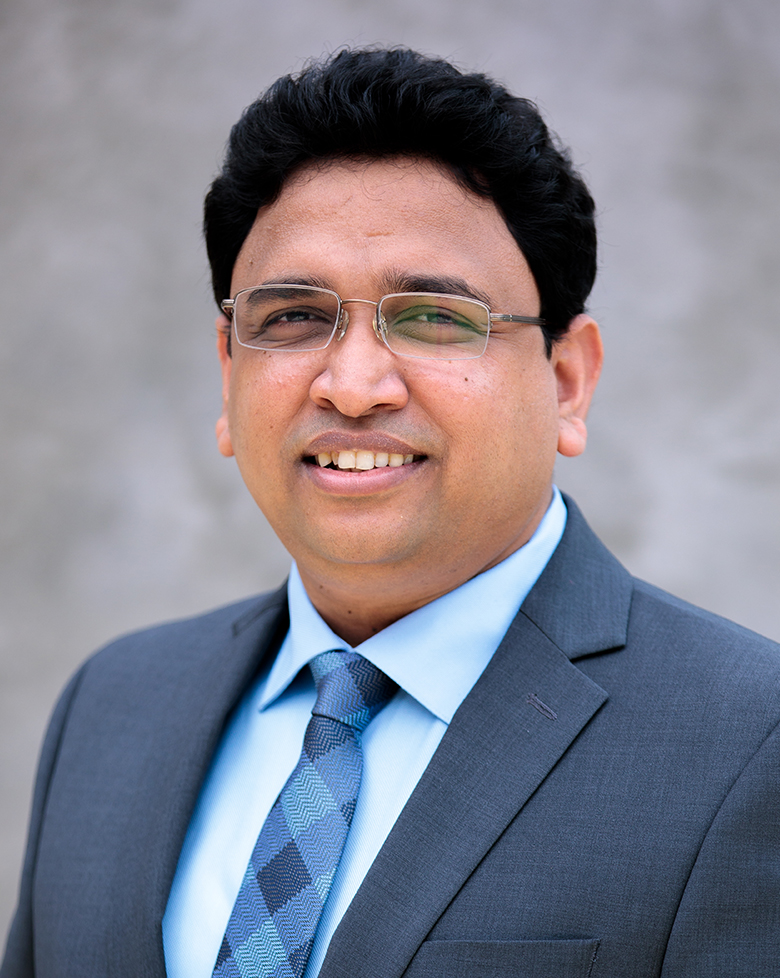
\includegraphics[width=1in,height=1.25in,clip,keepaspectratio]{photos/mizan.png}}]{Mizanur Rahman} (Senior Member, IEEE) received the B.Sc. degree in civil engineering from Bangladesh University of Engineering and Technology, Dhaka, Bangladesh, in 2008, and the M.Sc. and Ph.D. degrees in civil engineering (transportation systems) from Clemson University, Clemson, SC, USA, in 2013 and 2018, respectively. He is an Assistant Professor in the Department of Civil, Construction, and Environmental Engineering at The University of Alabama, Tuscaloosa, AL, USA. His research focuses on transportation cyber--physical systems/transportation digital twin, and transportation cybersecurity.
\end{IEEEbiography}

\vfill

\end{document}

